% intro: felix

This sections covers existing approaches to handle \cfgfiles{} as well as existing schema languages.
We compare them briefly and discuss why JSON schema is the most useful language for our approach.
As our research is of practical nature, we also consider gray literature like specifications of schemas or websites.

\subsection{Existing Approaches}\label{subsec:existing-approaches}
% felix
There exist several approaches that attempt to make maintaining \cfgfiles{} easier for the user.
Most of these approaches depend on the schema of the configuration file to be known.
Based on such a schema, it is possible to validate whether the config file adheres to the schema.
Findings from such a schema validation can be shown to the user, for example via syntax highlighting.
Additionally, the user can be assisted by means of graphical user interfaces.

% minye
\begin{listing}[!h]
\begin{minted}[frame=single,
               framesep=3mm,
               linenos=true,
               xleftmargin=15pt,
               tabsize=4]{js}
{
  "$id": "https://example.com
  /person.schema.json",
  "$schema": "https://json-schema.org
  /draft/2020-12/schema",
  "title": "Person",
  "type": "object",
  "properties": {
    "firstName": {
      "type": "string",
      "description": "first name."
    },
    "lastName": {
      "type": "string",
      "description": "last name."
    },
    "age": {
      "description": "Age",
      "type": "integer",
      "minimum": 0
    }
  }
}
\end{minted}
\caption{JSON schema example} 
\label{json-schema-example}
\end{listing}


\begin{listing}[!h]
\begin{minted}[frame=single,
               framesep=3mm,
               linenos=true,
               xleftmargin=15pt,
               tabsize=4]{js}
{
  "firstName": "John",
  "lastName": "Doe",
  "age": 21
}
\end{minted}
\caption{JSON example for the schema shown in Listing \ref{json-schema-example}} 
\label{json-example}
\end{listing}


\subsubsection{Schema Validation} % Keyuri

Schema validation is the process of checking whether a given data instance (e.g., a JSON, YAML or XML document) conforms to a predefined schema.
The specification for JSON schema validation can be found in the work of~\cite{JSON_schema_vailidation,JSONValidation}.
Listing~\ref{json-schema-example} is an exemplary JSON schema.
It could be used to validate the example instance shown in Listing~\ref{json-example}.

% todo note that we use AJV for schema validation (maybe in another section)

%We can also use a python library to validate.\ref{python_json_validation}

% \begin{figure}[!t]
% \centering
% 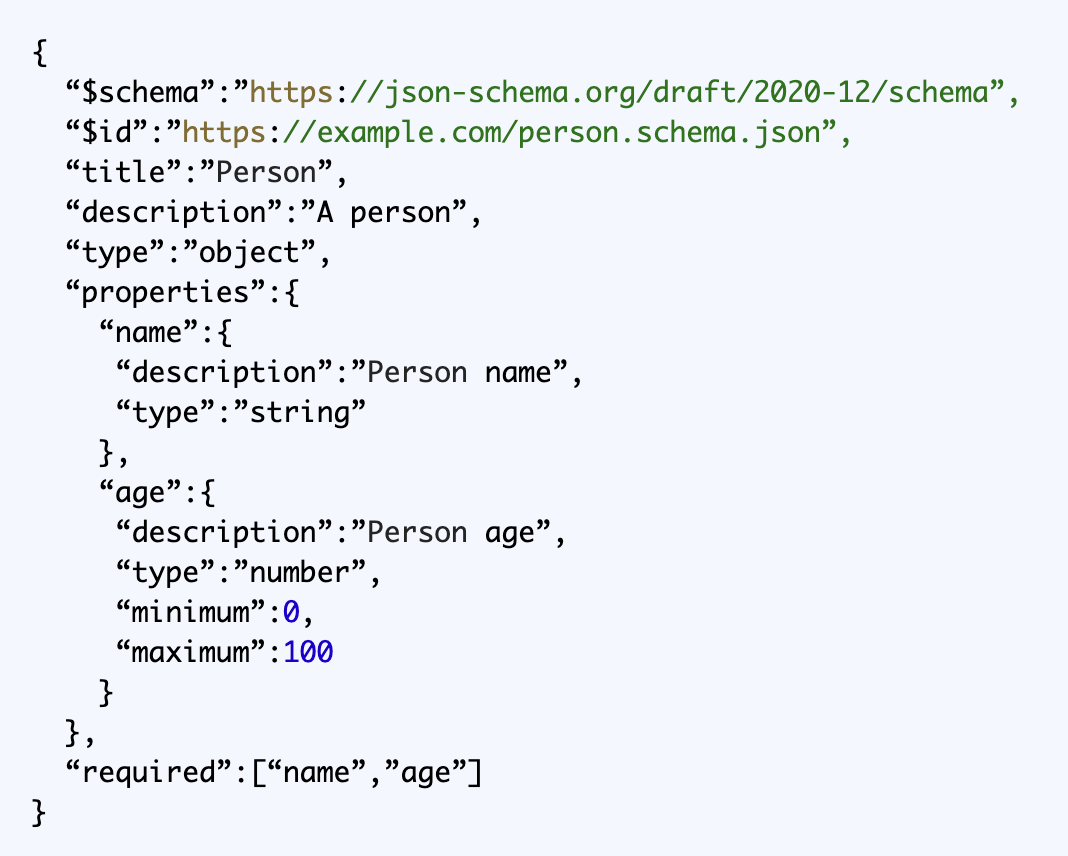
\includegraphics[width=2.5in]{schema_validation_demo.jpg}
% \caption{JSON schema demo}
% \label{schema_validation_demo}
% \end{figure}



% \begin{figure}[!t]
% \centering
% 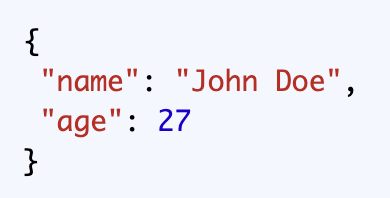
\includegraphics[width=2.5in]{instance_demo.jpg}
% \caption{Instance for validation}
% \label{instance_demo}
% \end{figure}

% \begin{figure}[!t]
% \centering
% 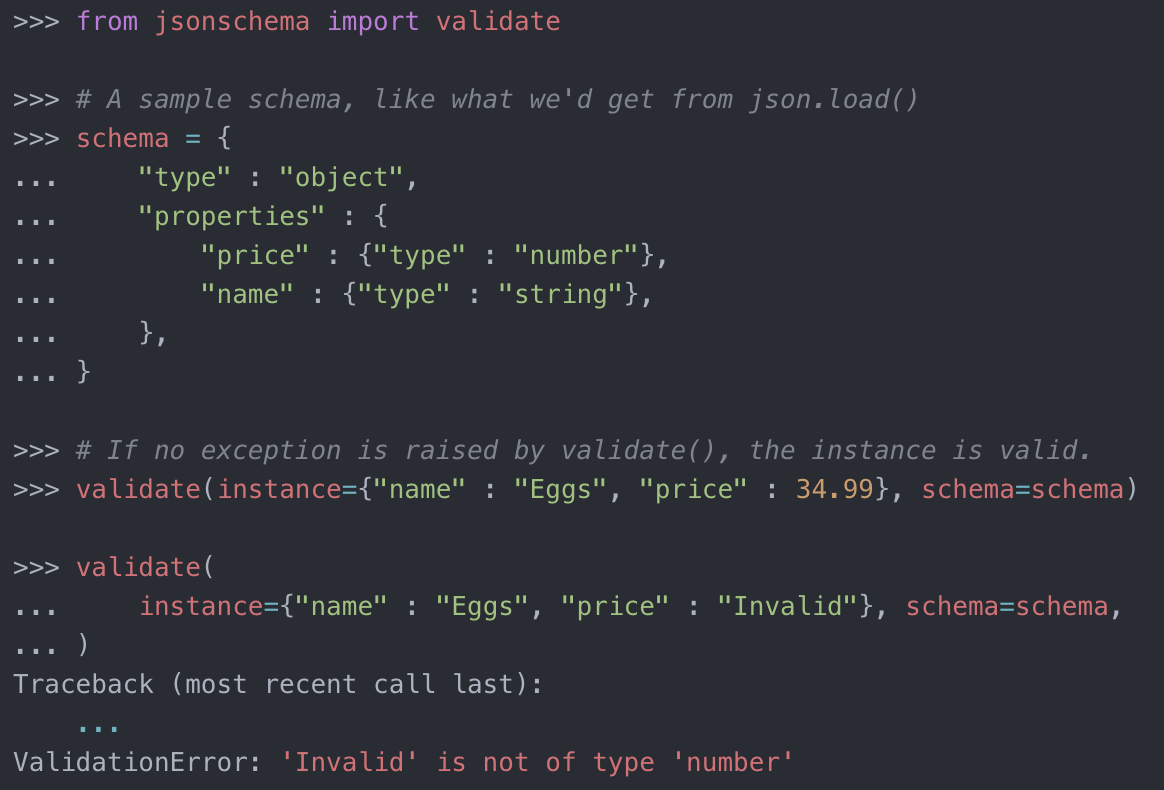
\includegraphics[width=2.5in]{python_json_validation.png}
% \caption{Validation using python library}
% \label{python_json_validation}
% \end{figure}

% todo: add paper about schema validation and possibly a small example

\subsubsection{Schema to GUI}
% minye and felix
Refers to the process of generating a graphical user interface (GUI) based on a predefined schema.
Such GUIs can assist the user in a multitude of ways, such as help by tooltips (Figure~\ref{fig:gui_advantage_tooltip}), Auto-Completion (Figure~\ref{fig:gui_advantage_autocomplete}) and Choice Selections (Figure~\ref{fig:gui_advantage_choiceselection}).

\begin{figure}[!t]
\centering

\includegraphics[width=2.5in]{figures/gui_advantage_tooltip}
\caption{Tooltip Assistance}
\label{fig:gui_advantage_tooltip}
\end{figure}

\begin{figure}[!t]
\centering
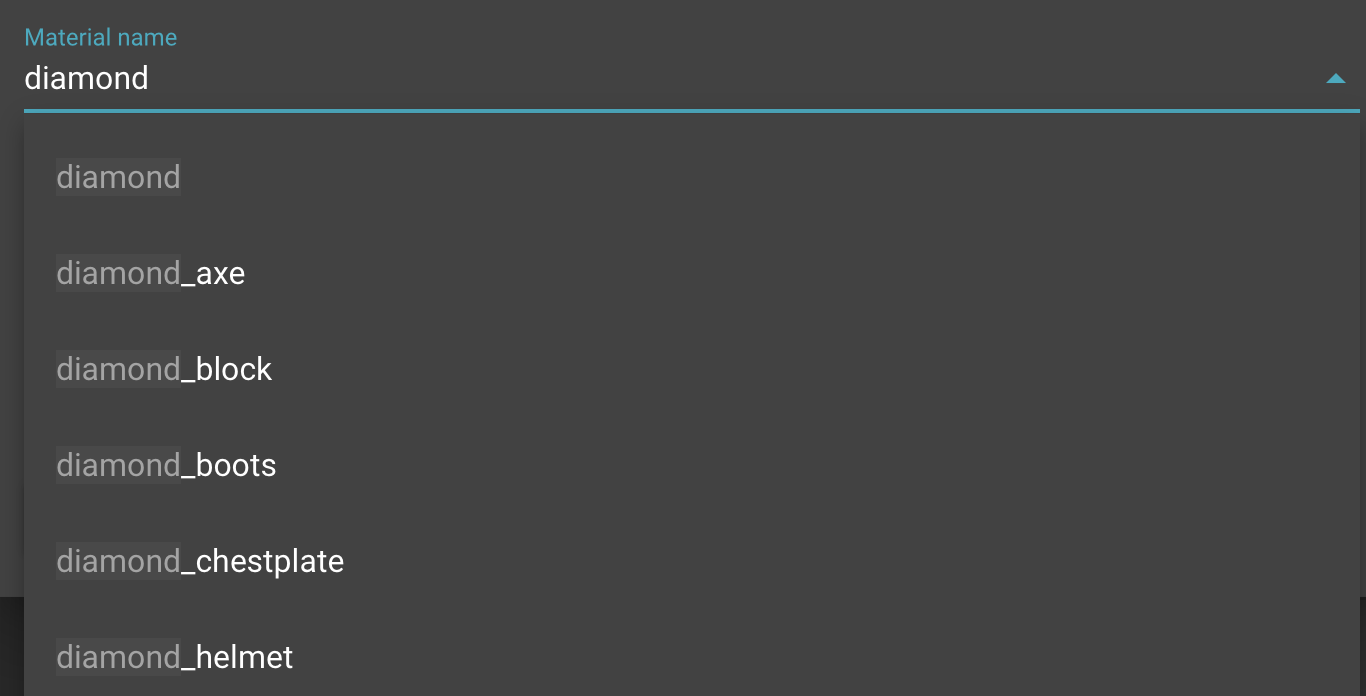
\includegraphics[width=2.5in]{figures/gui_advantage_autocomplete}
\caption{Auto-Completion}
\label{fig:gui_advantage_autocomplete}
\end{figure}

\begin{figure}[!t]
\centering
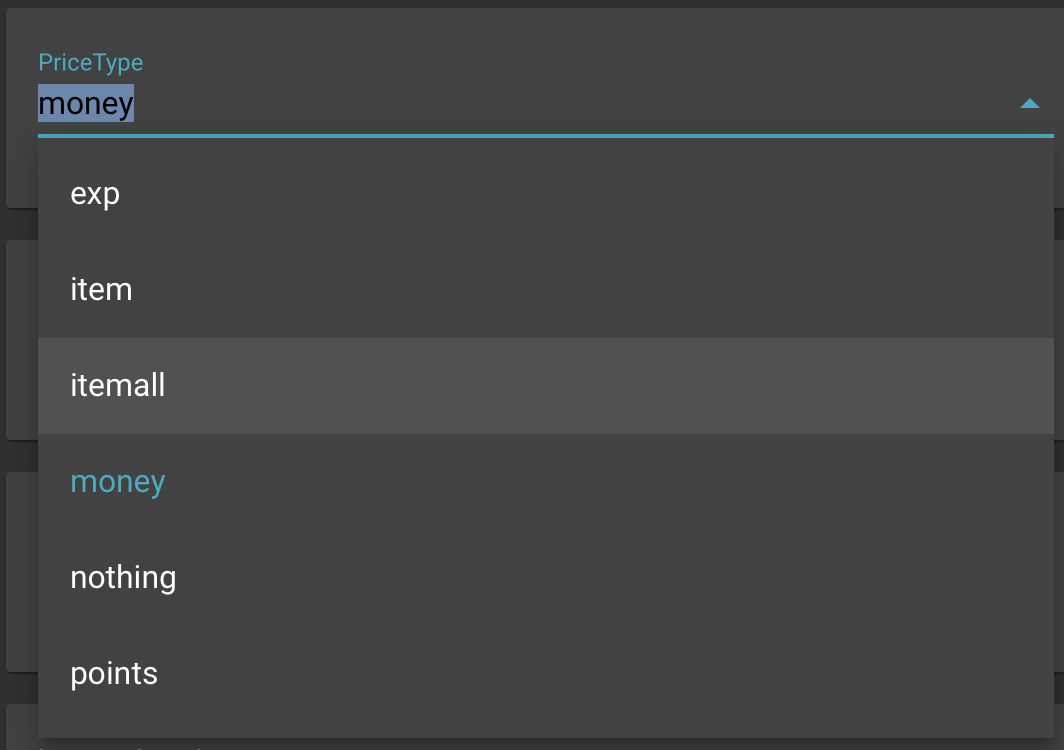
\includegraphics[width=2.5in]{figures/gui_advantage_choiceselection}
\caption{Choice Selection}
\label{fig:gui_advantage_choiceselection}
\end{figure}

% felix
By inherently adhering to the schema structure, with such GUIs configuration errors are avoided or at least significantly reduced.
Users that are not very familiar with the configuration schema profit most from the GUI assistance, but even experienced users tend to not remember every individual detail of the schema and benefit.

In the following, existing schema-to-UI approaches are listed.


% Minye
% todo more details
% adamant is specific for science context -> would be interesting
% it also extracts the unit from the description -> also interesting
% also how are they different from our approach?
\begin{enumerate}[label=(\alph*)]
    \item \textbf{Vue Form Generator}\cite{vueformgenerator}: is a schema-based form generator component for Vue.js.
    It can be extended with custom fields.
    At the time of writing this paper the tool was rated with most stars among web form generator projects. % todo reword maybe

    \item \textbf{JSON Forms}~\cite{JSONForms}: is a declarative framework for building form-based web UIs.
    It can be integrated with UI libraries or frameworks, such as Vue, React or Angular.

    \item \textbf{Adamant}~\cite{siffa2022adamant}: also is a JSON-schema based form generator, that supports any valid schema.
    It also supports schema validation.

\end{enumerate}

% paul

\subsection{Schema Languages}\label{subsec:schemalanguages}

Schema languages are formal languages that specify the structure, constraints, and relationships of data, for example in a database or in structured data formats.
Schema languages are text based, we do not consider any graphical modeling languages like UML.

For this work we consider using an existing schema language (or a subset of it), building on an existing schema language or introducing our own schema language.
The following sections describe existing schema languages.

% todo talk about ontology languages

%paul
\subsubsection{JSON schema}

JSON is a common data-interchange format for exchanging data with webservices, but also for storing documents in noSQL databases like MongoDB\@.
Because of the popularity of JSON, a demand for a schema for JSON documents evolved, which resulted in JSON schema~\cite{jsonSchema, jsonschemaJSONSchema}.

JSON schema has evolved to being the de-facto standard schema language for JSON documents. % todo citation, examples of usage
Schemas for many popular \cfgfile{} types exist. % todo give examples
JSON schema store\footnote{\url{https://www.schemastore.org/json/}} is a website that lists at the time of access 669 file types, for which they provide a JSON schema file.
The supported file types include for example Docker compose or OpenAPI files.
\cite{barbaglia, ChaeronySiffa2022} give further examples of JSON schema used in practice.


JSON and YAML documents are of a similar structure (JSON being a subset of YAML) and JSON schema can be applied on YAML documents too.
Some syntactical details of YAML can, however, not be expressed with JSON schema. % todo consider citatio

% felix
\subsubsection{XSD and DTD}
For XML the two de-facto standard schema languages are Document Type Definition (DTD)\cite{dtd_spec} and XML Schema Definition (XSD)\cite{xsd_spec}.
XSD is the newer and more expressive format of them and in large parts replaces and supersedes the more limited format DTD\cite{dtd_vs_xsd}.
It is recommended by W3C\cite{xsd_spec}.

Multiple more schema languages have been proposed and developed but are relatively unknown compared to XSD\cite{xml_schemas_1,xml_schemas_2}.

\subsubsection{CUE}\cite{cuelang} %Minye
(Configure, Unify, Execute) is a data validation and configuration language, which can be used with various data formats, such as JSON and YAML (it is a superset of both).
It has several use cases, especially in configuration and data validation.


\subsubsection{Apache Avro}% Keyuri
is an open source project that provides data serialization and data exchange services for Apache Hadoop.
It uses a JSON-based schema language~\cite{Apache-Avro}.

% TODO: reference to specs/website

% paul
\subsubsection{Other formats}

There exist other formats for defining data structures.
We also evaluated the GraphQL schema language and protobuf (also known as Protocol Buffers)
%protocol buffer?
The GraphQL schema language is used to define the data structures of GraphQL APIs~\cite{graphQL}.
Protobuf is a language for data serialization by Google~\cite{protobufProtocolBuffers}.

% Paul

\subsection{Evaluation of Schema Languages}\label{subsec:evaluation-of-schema-languages}

% todo Support for Reference


We evaluate several schema languages in how well they fit our use-case.
Ideally, the schema language is both popular and supported by numerous tools and libraries as well as having high expressiveness.

\subsubsection{Evaluation criteria} % evaluation by paul, some criteria ideas by felix

We evaluated the seven schema languages we mentioned in section~\ref{subsec:schemalanguages} based on the following criteria and metrics:
\begin{enumerate}
% metric: Stackoverflow question # with schema language as tag
    \item \textbf{Practical usage} --- Ideally our approach uses a schema language that already known by many developers. 
    As indicator of the practical usage we use the approximate search results on stackoverflow.com as metric.
    We aquire the results by querying the google search engine with the name of the schema language and ``site:stackoverflow.com'', which limits the search results to stackoverflow.com.
    This metric might also correlate with the complexity of the schema language as a more complex to use schema language will likely lead to more questions asked on the site. Nevertheless, we assume that a significantly higher number of results indicates that a language is more known than others.

    Additionally, we investigate how well the schema languages are supported by IDEs and code libraries.
    \begin{enumerate}
        \item \textit{Tool support} --- We used the 10 most popular IDEs\cite{mostpopularides} and checked if the IDE supports the schema language either natively or by a plugin. Support here means that either the IDE is capable of validating documents against a schema in the schema language or supports creating schema files, e.g. by using syntax highlighting for the schema language.
        % # node modules with schema language keyword....
        \item \textit{Library support} --- As we implement a web-based tool, we JavaScript or TypeScript bases tools are helpful for our approach, e.g. so we can reuse a package for schema validation. We investigate the number of node modules exist that are related to the schema languages by querying the node module search on \url{www.npmjs.com} with the name of the schema language.

    \end{enumerate}

    % # of cases fulfilled from below
    \item \textbf{Expressiveness} --- We evaluate how expressive each of the schema languages are, i.e. what possible constructs the language is able to express. We defines eight requirements on the language features that we consider helpful for our approach. The number of requirements a schema language fulfills is our metric that indicates how expressive the language is. Table~\ref{tab:comparison} reports the results. The eight requirements are:
    \begin{enumerate}
        \item \textit{Simple types} --- This is fulfilled if the schema language provides the possibility to define simple data types, at least strings, numeric types, and a boolean type. This is a fundamental feature required for our approach.
        \item \textit{Complex types} --- This is fulfilled if the schema language provides the possibility to define complex data types, at least records and arrays.
        This is crucial feature for our approach as configuration files are often structured data rather than plain key-value pairs.
        \item \textit{Descriptions} --- This is fulfilled if the schema language provides the possibility to add descriptions to fields. This is helpful in a schema-to-GUI approach as the description can be shown to the user, providing potential helpful information on how a field should be filled.
        \item \textit{Examples} --- This is fulfilled if the schema language provides the possibility to add example values. This is helpful in our approach as the example values can serve as placeholders in the GUI editor.
        \item \textit{Default values} --- This is fulfilled if the schema language provides the possibility to add default values which are assumed in an absence of a value. This often helpful information can be displayed to the user or used as placeholder values.
        \item \textit{Optional values} --- This is fulfilled if the schema language provides the possibility to declare values as optional or required. Often it is not necessary to provide all values in a configuration file, so it is helpful to mark fields as required or optional in the GUI editor.
        \item \textit{Constraints} --- This is fulfilled if the schema language provides the possibility possibility to constrain values of fields, e.g. maximum length of strings. To be exact, for this evaluation we required that at least two of the following constrained can be expressed by the schema language:
        \begin{itemize}
            \item The length of strings can be limited.
            \item The range of numeric types can be limited, e.g. to only positive values.
            \item The valid values of a field can be restricted to a finite amount of values (enumeration).
            \item The format of a string field can be constrained to a certain pattern.
        \end{itemize}
        This is a helpful feature for our approach as often not all possible values are valid for specific fields in configuration files.
        \item \textit{Conditions} --- This is fulfilled if the schema language provides the possibility to define conditional dependencies between fields. This is a advanced feature that is helpful because it allows to express for example that a particular field must be given only if another field has a specific value.
        \item \textit{References} --- This is fulfilled if the schema language provides the possibility to define reusable subschemas that can be referenced in other parts of the schema. This is often useful in practice to reuse common data structures.
    \end{enumerate}

    %\item \textbf{Support for XML, YAML, or JSON} ---  

    % For our approach we aim to use the same or at least a very similar editor for both editing the actual \cfgfiles and the schema files. Consequently, the schema language should be a subset of the language that the \cfgfiles are written in, i.e. the document language. For example JSON schema files are JSON files and JSON schema is used to validate JSON files, so here this criteria is fulfilled. In constrast, DTD is a schema language for validating XML files but a DTD file is not a valid XML file.

\end{enumerate}


    \begin{table*}[]
    \centering
    \caption{Evaluation of different schema languages\label{tab:all}}
        \begin{tabular}{@{}lrrrr@{}}
        \toprule
        \textbf{Schema language} &
          \textbf{\# Search results } &
          \textbf{IDE support} &
          \textbf{\# Node packages} &
          \textbf{Expressiveness} \\ \midrule
        JSON schema &
          245.000 &
          8 / 10 &
          4.536 & 8 / 8  \\
        XSD & 151.000 & 8 / 10 & 116 & 7 / 8 \\
        DTD & 69.700 & 9 / 10 & 34 & 5 / 8\\
        CUE & 10.500 & 4 / 10 & 97 & 7 / 8 \\
        Avro & 20.000 & 8 / 10 & 211 & 4 / 8 \\
        protobuf &  44.800 & 9 / 10 & 1.210 & 3 / 8\\
        GraphQl schema & 31.000 & 7 / 10 & 1.509 & 5 / 8\\ \bottomrule
        \end{tabular}
    \end{table*}
    %\label{fig:my_label}
%\end{figure}

% IDE                | JSON schema | XSD | DTD | CUE | Avro | protobuf | GraphQL schema |
% Visual Studio      | yes         | yes | yes | x   | yes  | yes      | yes            |
% Visual Studio Code | yes         | yes | yes | yes | yes  | yes      | yes            |
% Eclipse            | yes         | yes | yes | x   | yes  | yes      | x              |
% pyCharm            | yes         | yes | yes | yes | yes  | yes      | yes            |
% Android Studio     | yes         | yes | yes | yes | yes  | yes      | yes            |
% IntelliJ           | yes         | yes | yes | yes | yes  | yes      | yes            |
% NetBeans           | x           | yes | yes | x   | x    | yes      | x              |
% RStudio            | x           | x   | x   | x   | x    | x        | x              |
% Atom               | yes         | x   | yes | x   | yes  | yes      | yes            |
% Sumblime Text      | yes         | yes | yes | x   | yes  | yes      | yes            |
% ======================================================================================|
%                    | 8 / 10      | 8   | 9   | 4   | 8    | 9        | 7              |

\begin{table*}
    \centering
    \caption{Comparison of expressiveness of different schema languages
    \label{tab:comparison}}
    \begin{tabular}{@{}lllllllllr@{}}
         \toprule
        \textbf{Schema language} &
          \thead{Simple \\ types} &
          \thead{Complex \\ types} &
          \thead{Descriptions} &
          \thead{Example \\ values} &
          \thead{Default \\ values} &
          \thead{Optional \\ values} &
          \thead{Constraints} &
          \thead{Conditions}  &
          \thead{Result}\\ \midrule
        JSON schema &
          \checkmark &
          \checkmark &
          \checkmark &
          \checkmark &
          \checkmark &
          \checkmark &
          \checkmark &
          \checkmark & 8 / 8\\ 
        XSD &
          \checkmark &
          \checkmark &
          \checkmark &
          x &
          \checkmark &
          \checkmark &
          \checkmark &
          \checkmark\footnote{using assertions}& 7 / 8 \\
        DTD &
         \checkmark &
         \checkmark &
         x &
         x &
         \checkmark &
         \checkmark &
         x &
         \checkmark & 5 / 8\\
        CUE &
         \checkmark &
         \checkmark &
         \checkmark &
         (\checkmark)\footnote{only comments} &
         x &
         \checkmark &
         \checkmark &
         \checkmark & 7 / 8\\
        Avro &
         \checkmark &
         \checkmark &
         x &
         x & 
         \checkmark &
         \checkmark \footnote{Only allowing nullability, no distinction to absent values} &
         x &
         x & 4 / 8\\
        protobuf &
            \checkmark &
            \checkmark &
            x &
            x &
            x &
            \checkmark &
            x &
            x& 3 / 8 \\
        GraphQL schema &
         \checkmark &
         \checkmark &
         \checkmark &
         x &
         \checkmark &
         \checkmark &
         x &
         x & 5 / 8\\
          \bottomrule
    \end{tabular}
\end{table*}

% paul
\subsubsection{Evaluation results}

Table~\ref{tab:all} shows the results of our evaluation.
We come to the conclusion that JSON schema is sufficiently popular and expressive that we choose to use it as the schema language for our approach.
The other schema languages are either less expressive or less popular.

% paul

\subsection{JSON schema versions}\label{subsec:json-schema-versions}

JSON schema has had 10 different drafts over the years, the newest being draft 2020--12~\cite{jsonschemaJSONSchema}.
In real-world schemas we cannot expect schemas to all have the newest version.
Baazizi et al.~\cite{baazizi2021empirical} investigated over 82.000 open-source schemas in 2021, where they found that most of them are using draft 4, which was released in 2013.
As the different drafts are not necessarily compatible with each other, tools supporting one draft become outdated when a new draft releases.
However, Viotto et al.~\cite{Viotti_Lagoni_2023} provide a library for migration schemas from older versions to the newest draft without loss of information.
Thus, our tool only needs to support the newest draft directly.
If a user uses a schema from an older draft, we first migrate it to the newest draft internally.

% paul

\subsection{Schema inference}\label{subsec:schema-inference}

Schema inference is the process of deriving a schema from existing data.
For our use case, this means inferring JSON schema from JSON documents.
Frozza et al.~\cite{8424731} and Klettke et al.~\cite{klettke} present algorithms for JSON schema inference from JSON data of NoSQL data storages.
Baazizi et al.\cite{Baazizi2019} also investigate schema inference from massive data sets but their approach uses its own type system rather than JSON schema.

In our tool we only aim to infer a schema from a single sample, as an optional assisting feature for our users, for which various libraries exist~\cite{githubGitHubJsonsystemspublic, githubGitHubSaasquatchjsonschemainferrer, probst_siegel_2023}.